\documentclass[%
12pt, %
final, % 
oneside, % 
onecolumn, %  
centertags]{article} % относится к классу article и размер шрифта 12 пунктовб, {article: статья, report: отчеты и диссертации, book: книга, letter: письмо}

% \usepackage{fontspec}
 
% \setmainfont{Times New Roman}

% \documentclass[a4paper, 12pt]{report}

\topmargin= -30pt % насколько сверху будет страница
\textheight= 650pt


\usepackage[utf8]{inputenc} % задает кодировку, utf-8 кодировка, включающая в себя знаки почти всех языков мира
\usepackage[english]{babel} % подключает необходимые языки, основным языком является английский

\selectlanguage{english} % настройки будут на английском, но писать будет на русском

\usepackage{euscript}
\usepackage{supertabular}

\renewcommand{\baselinestretch}{1.0} 

\usepackage[colorlinks=true,linkcolor=blue,unicode=true,urlcolor = blue]{hyperref} %hypered
\usepackage[pdftex]{graphicx} % для графики

\usepackage{amsthm, amssymb, amsmath, amsfonts} % математический пакет, математические шрифты
\usepackage{textcomp}
\usepackage[noend]{algorithmic}
\usepackage[ruled]{algorithm}
\usepackage{lipsum}
\usepackage{indentfirst}
\usepackage{babel}
\usepackage{pgfplots}
\usepackage{setspace}
\usepackage{xcolor}
\usepackage{hyperref}
\usepackage{subfigure}

\setcounter{secnumdepth}{5}
\setcounter{tocdepth}{5}
\newcommand\simpleparagraph[1]{%
  \stepcounter{paragraph}\paragraph*{\theparagraph\quad{}#1}}
\usepackage{listings}
% \usepackage{xcolor}
%\usepackage{minted}

\lstset { %
     language=C++,
     backgroundcolor=\color{black!5}, % set backgroundcolor
     basicstyle=\footnotesize,% basic font setting
}


\linespread{1.0} 
\setlength{\parindent}{2.4em}
\setlength{\parskip}{0.1em}

\pgfplotsset{compat=1.9}
\pgfplotsset{model/.style = {blue, samples = 100}} 
\pgfplotsset{experiment/.style = {red}}

\theoremstyle{plain}
\binoppenalty=10000

\newtheorem{theorem}{Theorem}[section] % theorem

\theoremstyle{definition}
% \newtheorem{definition}{Определение}[subsection]
\newtheorem{definition}{Definition}[subsection]

\theoremstyle{remark}
% \newtheorem{remark}{Замечание}[section]

% \newtheorem{corollary}{Следствие}

% \newtheorem{proposition}{Proposition}

% \newtheorem{example}{Пример}

% \newtheorem{lemma}{Лемма}[section]

\renewcommand*{\proofname}{Proof}

\graphicspath{ {./images/} }


% \usepackage{amsmath,amsfonts,amssymb, setspace}  % Разнообразные математические команды и значки
% \usepackage{indentfirst}     % Отступ в первом абзаце

% \pagestyle{empty}
\usepackage[left=2.5cm, right=1.5cm, top=2.5cm, bottom=2.5cm]{geometry}
\usepackage[medium]{titlesec}
\usepackage{graphicx}
% \graphicspath{ {./images/} }

\begin{document}

	\begin{titlepage} 
		\begin{center}
		\textbf{}\\[2.0cm]
		\LARGE FEDERAL STATE AUTONOMOUS EDUCATIONAL INSTITUTION OF HIGHER EDUCATION \\[0.5cm]
		\Large ITMO UNIVERSITY \\[3cm]
		\LARGE Report\\
		\Large MPI. Assignments $12-13$ \\
		\Large Parallel algorithms for the analysis and synthesis of data \\[4cm]


		\begin{flushright}
		Performed by\\
		Aleksandr Shirokov\\
		J4133c\\
		Accepted by\\
		Petr Andriushchenko

		Deadline: 22.12.21
		\end{flushright}

		\vfill 

		{\Large {St. Petersburg}} \par
		{\Large {2021}}
		\end{center} 
	\end{titlepage}

\tableofcontents
\newpage


\section{Assignments}

\subsection{Assignment 12. MPI. Delayed interactions. Scheme of an iterative method 
with exchange over a ring topology using pending requests.}

\subsubsection{Formulation of the problem}

MPI allows for non-blocking operations to form whole packets of requests for communication operations \textsc{MPI\_Send\_init} and \textsc{MPI\_Recv\_init} , which are started by the \textsc{MPI\_Start} or \textsc{MPI\_Startall} functions.

Checking for completion of execution is performed by conventional means using the functions of the \textbf{WAIT} and \textbf{TEST} families.

Find and fix errors in \textsc{Assignment12.c}, add the for loop. When should you use a loop?


\subsubsection{Example of launch parameters and output. Detailed description of solution}

Code for \textbf{assignment 12} is \href{https:\//github.com/aptmess/parallel_algorithms/blob/master/HT/hw_mpi/Assignment12.c}{here}.

Compilation example: \textsc{mpic++ -o ./cpf/12.o Assignment12.c}

Launch example: \textsc{mpirun --oversubscribe -np 10 ./cpf/12.o}

\begin{center}
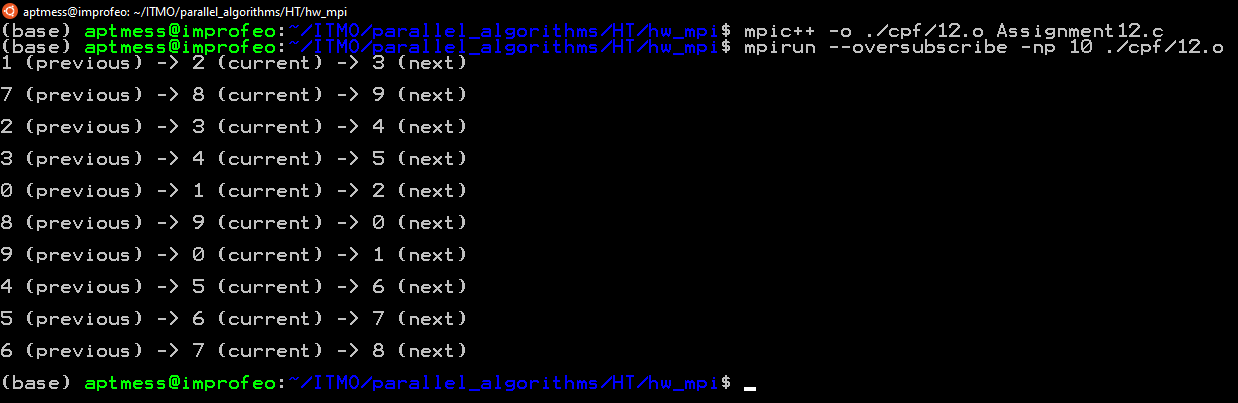
\includegraphics[scale=0.55]{12.png}
\end{center}

Let's move to the the code and explain how it works.

\begin{center}
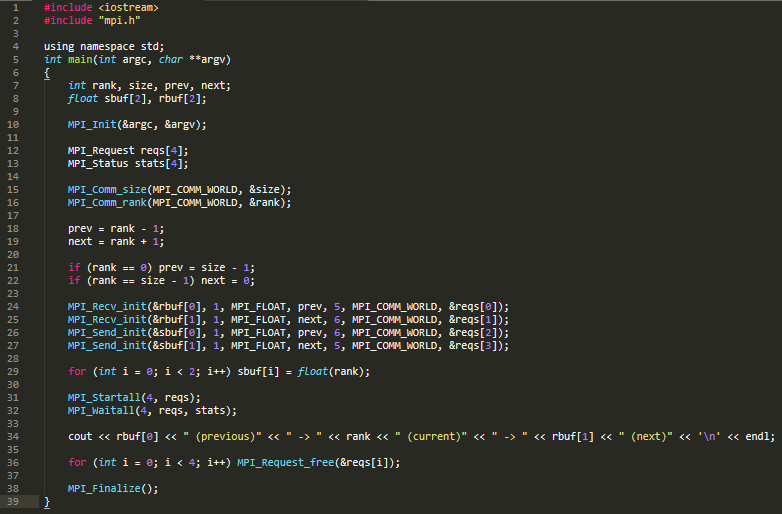
\includegraphics[scale=0.8]{12.code.png}

Assignment12 code
\end{center}

Firstly i wrote a whole program that can be compiled and works correctly as a ring topology as we can see on picture. As fixing errors in lines $24-27$ i have add by symbol \textsc{\&} address of variable \textsc{rbuf} and \textsc{sbuf} (also i have created float arrays with the same names), also do the same for \textsc{reqs}. In lines $26-27$ we can see that there is no values in array \textsc{sbuf}, so for loop is for mapping float value of rank to each piece of array (line $29$). Inside for loop there is no need to start sending and recieving messages on each iteration - we should do it only ones as i did it in lines $31-32$. After that i displayed information in ring topology and used for loop for function \textsc{MPI\_Request\_free} to free inactive persistent requests created with either \textsc{MPI\_Recv\_init} or \textsc{MPI\_Send\_init} and friends. All that i said is the answer on question when should we use loop: free inactive requests and may be for initialzing data to send. That's all, program works correctly and errors are fixed. 


\newpage
\subsection{Assignment 13. MPI. Collective process interactions. Barrier.}

\subsubsection{Formulation of the problem}

Find out which process will perform the multiplication of two $500 \times 500$ square matrices faster.

Complete the code \textsc{Assignment13.c}. You can use the necessary code from the previous assignments.


\subsubsection{Example of launch parameters and output. Detailed description of solution}

Code for \textbf{assignment 13} is \href{https:\//github.com/aptmess/parallel_algorithms/blob/master/HT/hw_mpi/Assignment13.c}{here}.

Compilation example: \textsc{mpic++ -o ./cpf/13.o Assignment13.c}

Launch example: \textsc{mpirun --oversubscribe -np 5 ./cpf/13.o 500}

\begin{center}
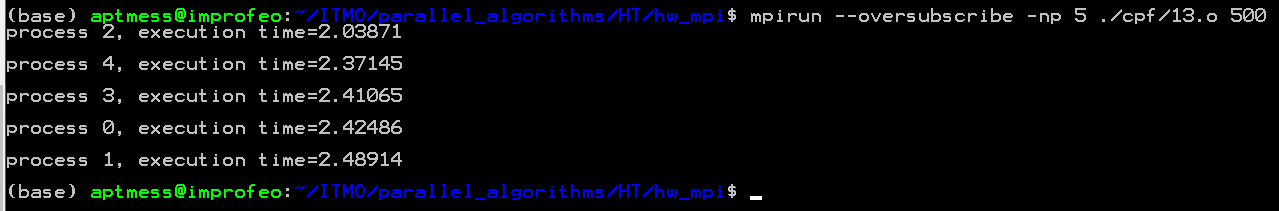
\includegraphics[scale=0.55]{13.png}
\end{center}

Let's move to the the code and explain how it works.

\begin{center}
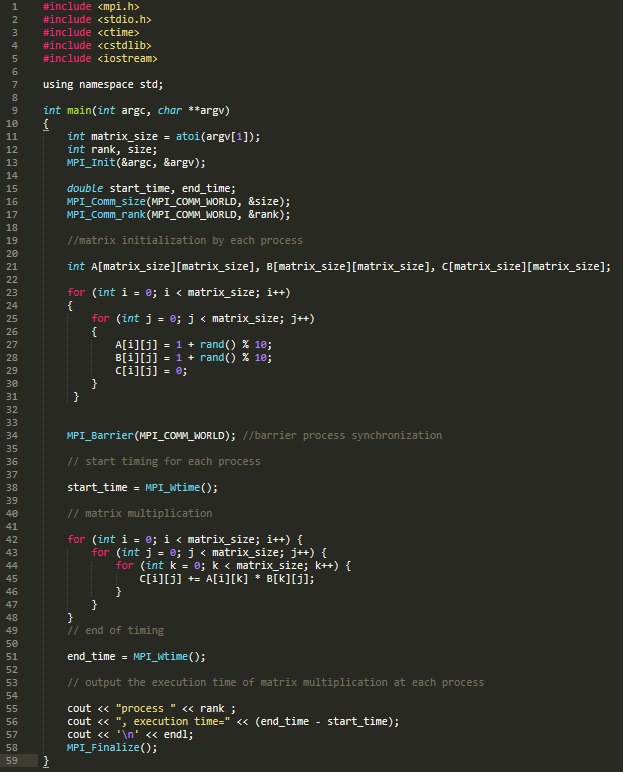
\includegraphics[scale=0.8]{13.code.png}

Assignment13 code
\end{center}

What should we need was written in file by comments, by job was to fill the gaps as code. Firstly i initialize matrices $A$ and $B$ with the same seed for each process with random integers from $1$ to $10$ and matrix $C$ by null values. Next there are a barrier function which is waiting when all processes initialize their matrices, after that we start timing for eahc process, do known matrix multiplication algorithm, end timing and show execution time of matrix multiplication at each process and understand which process performed faster. In our example it is process with rank $2$. Program works correcly and algorithm is explained.

\subsection{Appendix}

The link to the sourse code which is placed on my \href{https://github.com/aptmess/parallel_algorithms}{github}.


\end{document}